\documentclass{beamer}

%\documentclass{article}
%\usepackage{beamerarticle}

\usepackage[utf8]{inputenc}

%\usetheme{Warsaw}
%\usetheme{Hannover}
\usetheme{Berkeley}
%\usecolortheme{lily}
\setbeamertemplate{theorems}[numbered] 
%\setbeamertemplate{theorems}[ams style]
\date{}

%\theoremstyle{plain}

\usepackage{lmodern}
\usepackage[T1]{fontenc}
\usepackage[utf8]{inputenc}
\usepackage[french]{babel}
\usepackage{tikz,tkz-tab}
\usepackage{graphics}
\usepackage{pstricks,pst-node,pst-tree}
\usepackage{multicol}
\usepackage{array}

\uselanguage{French}
\languagepath{French}

\newtheorem{proposition}[theorem]{\translate{Proposition}}
%\newtheorem{example}[theorem]{\translate{Example}}
\newtheorem{demonstration}[theorem]{Démonstration}
\newtheorem{remark}[theorem]{Remarque}

\newcommand{\R}{\mathbb{R}}

\title{Probabilités.}


\begin{document}
  
  \begin{frame}
    
    \titlepage
   % \maketitle
    
  \end{frame}
  
  \section{Définition}
 
  \begin{frame}
  
  \begin{definition}
  Une \textbf{probabilité} sur un \uncover<2,3,4,5,6,7>{univers} fini 
  $\Omega=\lbrace \omega_1,...,\omega_n \rbrace$ est la donnée
  d'une fonction $$P:\Omega \to \uncover<3,4,5,6,7>{[0;1]} \textrm{ telle que }
  \sum_{i=1}^n P(\omega_i)=\uncover<4,5,6,7>{1}$$
  
  On appelle \textbf{éventualité} ou \textbf{issue} un \uncover<5,6,7>{élément} 
  $\omega_i$ de $\Omega$.
  
  On appelle \textbf{événement} une \uncover<6,7>{partie} $A$ de $\Omega$, i.e un ensemble d'issues.
  
  On peut étendre $P$ aux événements:
  $$
  \begin{array}{llll}
		P:&\mathcal{P}(\Omega) &\to& [0,1] \\
		  &A                   & \mapsto &
		  P(A)=\uncover<7>{\sum\limits_{\omega \in A} P(\omega)}\\
  \end{array}
  $$
   
  \end{definition}
  
  \end{frame}
  
  \begin{frame}
  
  Modéliser le caractère aléatoire d'une expérience consiste à définir une fonction de
  \uncover<2,3,4,5,6,7,8,9,10,11>{probabilité}
  sur l'ensemble des issues de cette expérience.
  
   \begin{example} 
   On réalise un lancer d'un dé équilibré à $6$ faces.
   
   Quelle est la probabilités d'obtenir un résultat pair ?
   
   $\Omega=\uncover<3,4,5,6,7,8,9,10,11>{\lbrace 1,..,6 \rbrace$}, $A=
   \lbrace \omega \in \Omega / \uncover<4,5,6,7,8,9,10,11>{\omega \textrm{ est pair}} \rbrace=
   \lbrace \uncover<5,6,7,8,9,10,11>{\omega
    \textrm{ est pair}} \rbrace =\lbrace \uncover<6,7,8,9,10,11>{2;4;6} \rbrace$.
    
    Le dé étant équilibré, il y a \uncover<7,8,9,10,11>{équiprobabilité} et 
    $P(2)=P(4)=P(6)=\uncover<8,9,10,11>{\frac{1}{6}}$.
    $P(A)=P(2)+P(4)+P(6)=\uncover<9,10,11>{3} \times \frac{1}{6}=\uncover<10,11>{\frac{1}{2}}$.
    
    
    De façon équivalente, comme il y a équiprobabilité, on peut écrire:
    
    $P(A)=\frac{\uncover<11>{Card(A)}}{\uncover<11>{Card(\Omega)}}=\frac{3}{6}=\frac{1}{2}$ où Card signifie le nombre d'éléments.

  \end{example}
  
  \end{frame}
  
  \section{Suites d'experiences aléatoires} 
    
  \begin{frame}
  \begin{theorem}
      Lorsqu'une expérience aléatoire est 
      constituée d'une suite de n expériences aléatoires (ou épreuves), 
      on peut la représenter par un \uncover<2,3,4,5>{arbre pondéré}. 
      Une issue est la liste ordonnée des résultats que l'on peut 
      représenter par un \uncover<3,4,5>{chemin} de l'arbre.
      
      \begin{itemize}
      
      \item Loi des chemins:
       
       La probabilité d'une issue est \uncover<4,5>{le produit} des 
       probabilités inscrites sur chacune des arêtes
       constituant le chemin associé à cette issue.
       
       \item Loi des noeuds:
       
       La somme des probabilités inscrites sur les arêtes
       issues d'un même noeud vaut \uncover<5>{1}.
       
       
      \end{itemize}

   \end{theorem}
  \end{frame}
  
   \begin{frame}
   \begin{definition}
   On dit qu'une expérience aléatoire est constituée d'une suite d'épreuves \textbf{indépendantes},
   \textbf{identiquement distribuées} si chaque épreuve ne dépend pas des résultats des épreuves 
   précédentes, c'est à dire si les issues possibles sont les mêmes et avec la même répartition
   de probabilités.
  \end{definition}
  
    \end{frame}
     
   \begin{example}[Page 319]
   
   \begin{itemize}

    \item 
    \href{https://github.com/mathlorgues/math1sd1516/blob/master/Chapitres/6.%20Probabilit%C3%A9s/Images/tirageRemise.png}
  {Tirage avec remise} (épreuves indépendantes, identiquement distribuées)
    dans une urne contenant 2 boules bleues, 2 rouges et une noire.

  \item Représentation de l'expérience par
  \href{https://raw.githubusercontent.com/EdisonLorgues1SD1617/Math1SD1617/master/Donn%C3%A9es/Chapitres/6.%20Probabilit%C3%A9s/Images/arbrePondere.png}
   {un arbre pondéré}.

   \end{itemize}
  % \center{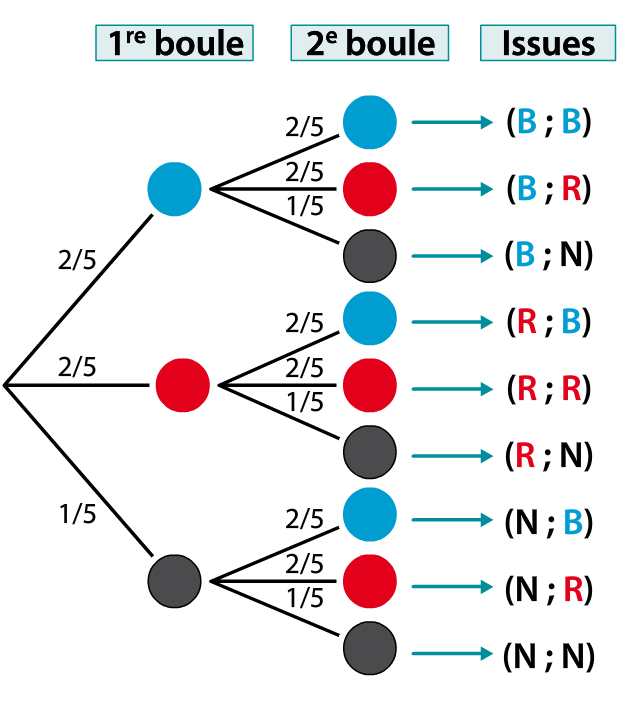
\includegraphics[scale=0.2]{../Images/issues.png}}
  \end{example}

  
  
  \section{Variables aléatoires}
  
  \subsection{Définition}
  
  \begin{frame}
   \begin{definition}
      Etant donnée une expérience aléatoire dont l'univers (l'ensemble des issues possibles) est 
      $\Omega$. Définir une \textbf{variable aléatoire} (réélle) $X$ sur $\Omega$ consiste à associer à
      chaque issue un nombre réél. Autrement dit, $X$ est une \uncover<2,3,4>{fonction}
      $X:\uncover<3,4>{\Omega} \to \uncover<4>{\mathbb{R}}$.
   \end{definition}
  \end{frame}
  
  \begin{frame}
    \begin{example}
   
   On définit, sur l'expérience aléatoire de l'exemple précédent, la variable (aléatoire) qui
   associe à un tirage le nombre de boule rouge obtenue.
   
   Il y a seulement \uncover<2,3>{$3$} valeurs possibles pour cette variable aléatoire: \uncover<3>{$0,1,2$}.
  
   \end{example}
  \end{frame}
  
  \subsection{Loi de probabilité}
  
  \begin{frame}
  \begin{definition} 
    
   Soit $\Omega$ un univers muni d'une fonction de probabilité $P:\Omega \to [0;1]$.
   
   Soit $X$ une variable aléatoire $X:\Omega \to \mathbb{R}$ avec $x_i,i=1,..,k$ ses différentes 
   valeurs.
   
   \'Etablir la \textbf{loi de probabilité} de $X$ consiste à associer à chaque valeur $x_i$ la probabilité
   de l'événement \uncover<2>{$X=x_i$}.
   
   \end{definition}
   
   \end{frame}
   
   \begin{frame}
   \begin{example}
    Soit $X$ la variable aléatoire qui compte le nombre de boules rouges tirées, de l'exemple précédent.

    \begin{multicols}{2} 
 
 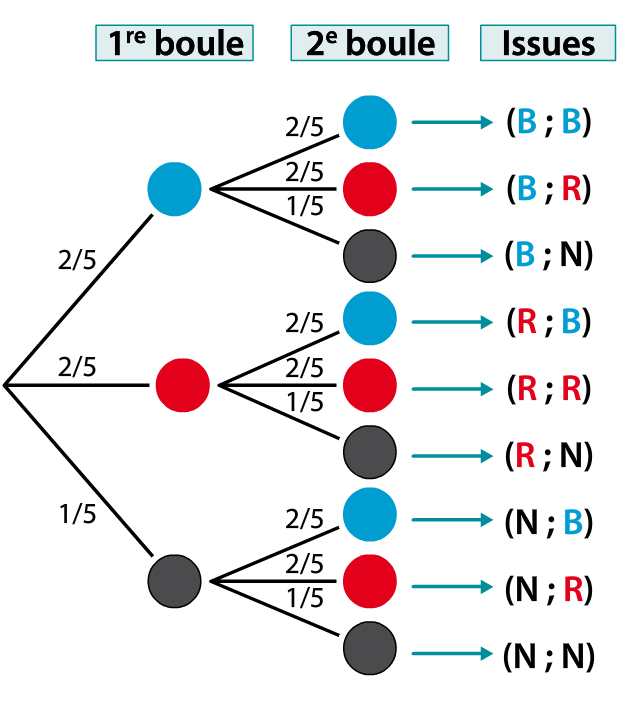
\includegraphics[scale=0.3]{../Images/issues.png}
 
\columnbreak 
 
 \tiny 
\begin{tabular}{ll}
    $P(X=0)$\\
    $=P(\uncover<2,3,4,5,6,7,8,9,10>{\lbrace(B;B);(B;N);(N;B);(N;N)\rbrace})$ \\
    $=\uncover<3,4,5,6,7,8,9,10>{P(B;B)+P(B;N)+P(N;B)+P(N;N)}$\\
    $=\uncover<4,5,6,7,8,9,10>{(\frac{2}{5})^2}+\uncover<5,6,7,8,9,10>{\frac{2}{5}\frac{1}{5}}+\uncover<6,7,8,9,10>{\frac{1}{5}\frac{2}{5}}+
    \uncover<7,8,9,10>{(\frac{1}{5})^2}=\uncover<8,9,10>{\frac{9}{25}}$\\
    \end{tabular}
\uncover<9,10>{    
\begin{tabular}{ll}
    $P(X=1)$\\
    $=P(\lbrace(B;R);(R;B);(R;N);(N;R)\rbrace)$ \\
    $=P(B;R)+P(R;B)+P(R;N)+P(N;R)$\\
    $=(\frac{2}{5})^2+(\frac{2}{5})^2+\frac{2}{5}\frac{1}{5}+\frac{1}{5}\frac{2}{5}=\frac{12}{25}$\\
    \end{tabular} 
    
\begin{tabular}{ll}
    $P(X=2)$\\
    $=P(\lbrace(R;R)\rbrace)$ \\
    $=P(R;R)$\\
    $=(\frac{2}{5})^2=\frac{4}{25}$\\
    \end{tabular} 
}
\uncover<10>{
\renewcommand{\arraystretch}{1.5}
 $$
\begin{array}{|c|c|c|c|}

\hline
    x_i&0&1&2\\
    \hline
    P(X=x_i)&\frac{9}{25}&\frac{12}{25}&\frac{4}{25}\\
    \hline
    \end{array} 
$$    
} 
\end{multicols}
\end{example}
   \end{frame}
   
\subsection{Paramètres d'une variable aléatoire}
               
Une loi de probabilité d'une variable aléatoire $X$:
 $$
\begin{array}{|c|c|c|c|c|}

\hline
    x_i&x_1&x_2&...&x_k\\
    \hline
    P(X=x_i)&p_1&p_2&...&p_k\\
    \hline
    \end{array} 
$$ 

est l'estimation des fréquences obtenues en faisant des statistiques sur un grand
nombre de réalisations de l'expérience aléatoire:
 $$
\begin{array}{|c|c|c|c|c|}

\hline
    x_i&x_1&x_2&...&x_k\\
    \hline
    f_i&f_1&f_2&...&f_k\\
    \hline
    \end{array} 
$$ 
 
De même que nous avons défini les paramêtres moyenne, variance et écart-type d'une série statistique, 
nous définissons espérance $E(X)$, variance $var(X)$ et écart-type $\sigma_X$ d'une variable aléatoire $X$.

\begin{frame}

  \begin{definition}[Paramètres d'une variable aléatoire] 
    
   $$E(X)=\sum^k_{\uncover<2,3,4,5,6,7,8>{i=1}} \uncover<3,4,5,6,7,8>{p_i x_i}
   =\uncover<4,5,6,7,8>{p_1 x_1+...+p_k x_k}$$
   
   $$Var(X)=E((X-E(X))^2)=\sum_{i=1}^k p_i \uncover<5,6,7,8>{(x_i-E(X))^2}$$
   
   $$Var(X)=E(X^2)-E(X)^2=\sum_{i=1}^k \uncover<6,7,8>{p_i x_i^2}-(\sum_{i=1}^k \uncover<7,8>{p_i x_i})^2$$
   
   $$\sigma_X=\uncover<8>{\sqrt{Var(X)}}$$
   \end{definition}
\end{frame}
  
\begin{frame}

\begin{example}
 
  On reprend l'exemple du tirage de boules de l'exemple précédent:

$
 \begin{array}{|c|c|c|c|}

\hline
    x_i&0&1&2\\
    \hline
    P(X=x_i)&\frac{9}{25}&\frac{12}{25}&\frac{4}{25}\\
    \hline
    \end{array} $

    $E(X)=\uncover<2,3,4,5,6,7,8,9,10,11,12,13,14,15,16,17,18,19>{0} \times 
    P(\uncover<3,4,5,6,7,8,9,10,11,12,13,14,15,16,17,18,19>{X=0})+
    \uncover<4,5,6,7,8,9,10,11,12,13,14,15,16,17,18,19>{1} \times 
    P(\uncover<5,6,7,8,9,10,11,12,13,14,15,16,17,18,19>{X=1})+
    \uncover<6,7,8,9,10,11,12,13,14,15,16,17,18,19>{2} \times 
    P(\uncover<7,8,9,10,11,12,13,14,15,16,17,18,19>{X=2})$
    
    $=\uncover<8,9,10,11,12,13,14,15,16,17,18,19>{\frac{12}{25}}+2 \times 
    \uncover<9,10,11,12,13,14,15,16,17,18,19>{\frac{4}{25}}=
    \uncover<10,11,12,13,14,15,16,17,18,19>{\frac{20}{25}}
    =\frac{4}{5}$
    
    $E(X^2)=\uncover<11,12,13,14,15,16,17,18,19>{0^2} \times P(X=0)+
    \uncover<11,12,13,14,15,16,17,18,19>{1^2} \times P(X=1)+
    \uncover<11,12,13,14,15,16,17,18,19>{2^2} \times P(X=2)$
    
    $=\uncover<12,13,14,15,16,17,18,19>{\frac{12}{25}+4 \times \frac{4}{25}}=
    \uncover<13,14,15,16,17,18,19>{\frac{28}{25}}$
    
    $Var(X)=\uncover<14,15,16,17,18,19>{\frac{28}{25}}-\uncover<15,16,17,18,19>{(\frac{4}{5})^2}=
    \frac{\uncover<17,18,19>{28}- \uncover<18,19>{16}}
    {\uncover<16,17,18,19>{25}}=\frac{12}{25}$
    
        $\sigma_X=\uncover<19>{\frac{2\sqrt{3}}{5}}\simeq 0.69$
\end{example}    
\end{frame}

  \begin{frame}
   \begin{theorem}
    Soit $X:\Omega \to \mathbb{R}$ une variable aléatoire. On note $aX+b$ la variable aléatoire
     telle que $(aX+b)(\omega)=aX(\omega)+b$.
     
     $$E(aX+b)=\uncover<2,3>{aE(X)+b}$$
     
     $$Var(aX+b)=\uncover<3>{a^2 var(X)}$$
   \end{theorem}
   \end{frame}

     \begin{frame}
   \begin{theorem}[Loi des grands nombres]
    
    Pour un grand nombre d'expériences aléatoires réalisées la moyenne (resp. l'écart-type)
    des valeurs observées pour $X$ est proche de \uncover<2,3>{l'espérance} 
    (resp. \uncover<3>{l'écart-type}) de $X$.
    
   \end{theorem}
   \end{frame}
   
 
   
    \section{Schéma de Bernoulli}
  \subsection{\'Epreuve de Bernoulli}
  \begin{frame}
  \begin{definition}[Schéma de Bernoulli d'ordre 1]
    Une \textbf{épreuve de Bernoulli} est une expérience aléatoire qui admet exactement deux issues:
    Succès et \uncover<2,3,4,5>{échec}.
    
    En associant à cette expérience aléatoire la variable $X$ qui vaut $1$ en cas de succès et 
    $0$ en cas d'échec, on obtient pour X la loi de probabilité suivante:
     
     \renewcommand{\arraystretch}{1.5}
 $$
\begin{array}{|c|c|c|}

\hline
    k&0&1\\
    \hline
    \uncover<3,4,5>{P(X=k)}&\uncover<4,5>{1-p}&p\\
    \hline
    \end{array} 
$$   
     On dit que $X$ suit une \textbf{loi de bernoulli} de paramètre \uncover<5>{$p$} et 
     on note $X \hookrightarrow B(p)$.
  \end{definition}
  \end{frame}
  
  \begin{frame}
   \begin{example}
    On lance un dé équilibré à 6 faces. On définit le succès par l'événement <<Obtenir 6>>.
    La variable aléatoire $X$ associée à cette épreuve de Bernoulli suit la loi de 
    \uncover<2,3,4>{Bernoulli de paramètre $\frac{1}{6}$}.
    
    $X \hookrightarrow B(\frac{1}{6})$
    
    \renewcommand{\arraystretch}{1.5}
     $$
\begin{array}{|c|c|c|}

\hline
    k&0&1\\
    \hline
    \uncover<3,4>{P(X=k)}&\uncover<4>{\frac{5}{6}}&\uncover<4>{\frac{1}{6}}\\
    \hline
    \end{array} 
$$
  
 \end{example}
 \end{frame}
 
 \begin{frame}
 \begin{proposition}
  Soit $X$ une variable aléatoire suivant une loi de bernoulli de paramètre $p$.
  $$E(X)=p$$ $$Var(X)=p(1-p)$$
  
  Démonstration:
  
  $E(X)=\uncover<2,3,4,5,6,7,8,9>{0} \times \uncover<3,4,5,6,7,8,9>{(1-p)}+ 
  \uncover<4,5,6,7,8,9>{1}\times \uncover<5,6,7,8,9>{p}=p$
  
  $E(\uncover<6,7,8,9>{X^2})=\uncover<7,8,9>{0^2} \times (1-p)+\uncover<7,8,9>{1^1} \times p=p$
  
  $Var(X)=\uncover<8,9>{E(X^2)}-\uncover<9>{E(X)^2}=p-p^2=p(1-p)$
 \end{proposition}
\end{frame}

  \begin{frame}
  
   \begin{example}
 Dans la situation de l'exemple précédent:
 
 $E(X)=\uncover<2,3,4,5>{p}=\uncover<3,4,5>{\frac{1}{6}}$
 
 $Var(X)=\uncover<4,5>{\frac{1}{6}} \times \uncover<5>{\frac{5}{6}}=\frac{5}{36}$.
  
 \end{example}
 \end{frame}
 
 \subsection{Schéma de Bernouilli d'ordre n}

 \begin{frame}
  
  \begin{definition}[Schéma de Bernoulli d'ordre $n$]
  On appelle \textbf{schéma de Bernoulli} d'ordre $n$ et de paramètre $p$, 
  l'expérience aléatoire constituée
  par une suite de $n$ épreuves de Bernoulli de paramètre $p$, 
  \uncover<2,3,4>{indépendantes} et \uncover<2,3,4>{identiquement distribuées}.
  
  Le résultat de l'expérience est la liste des $n$ résultats représentée par un mot
  $$R_1R_2...R_n$$
  où $R_i= S$ ou $\overline{S}$.
  
  On peut représenter l'expérience par un \uncover<3,4>{arbre pondéré} et la probabilité d'une issue est:
  $$p^k(1-p)^{n-k}$$ où $k$ est \uncover<4>{le nombre de succès}.
 \end{definition}

 \end{frame}
 
 \begin{frame}
   \begin{example}
 On réalise $3$ lancers successifs d'un dé équilibré, en considérant à chaque lancer <<obtenir 6>>
 comme le succès. La suite de ces trois épreuves de Bernoulli peut être représentée par l'arbre pondéré
 suivant:
 
  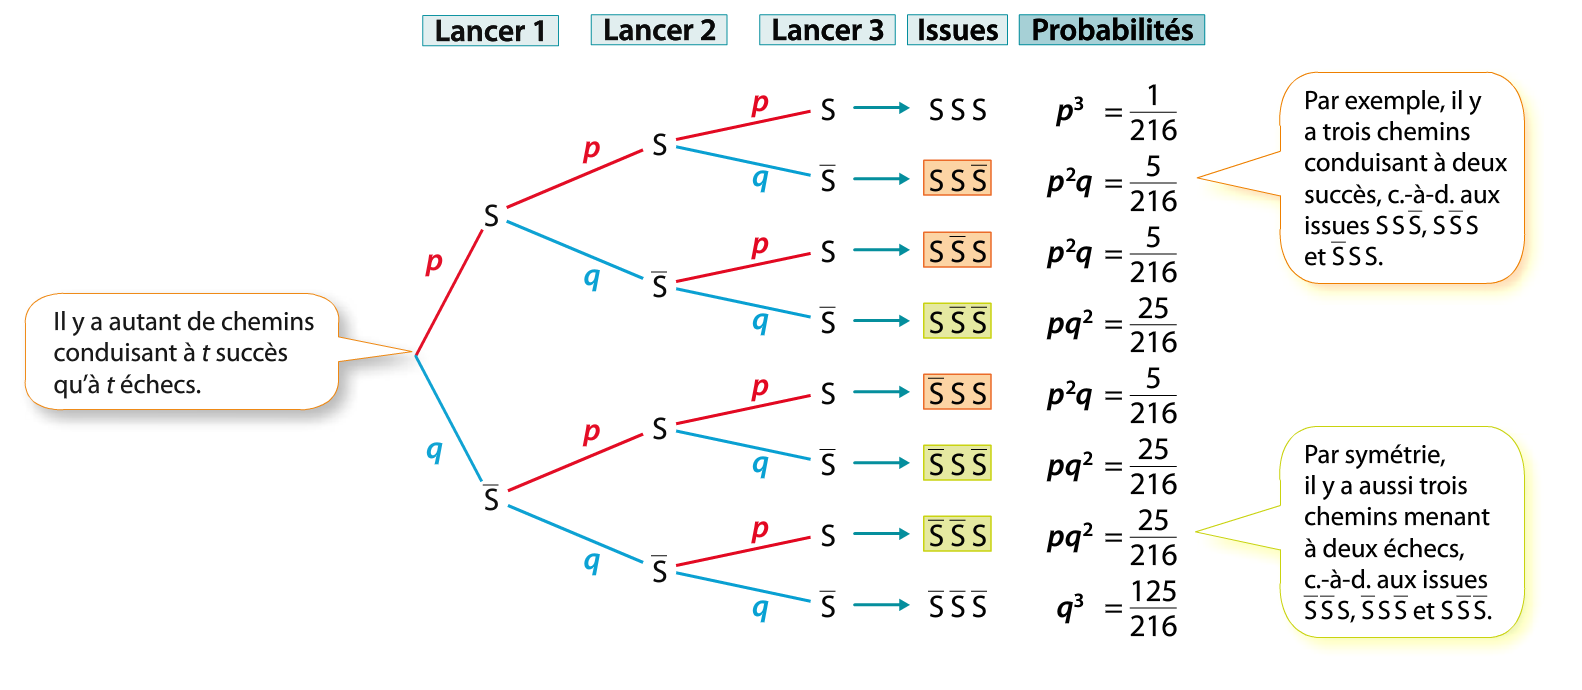
\includegraphics[scale=0.3]{../Images/arbreBinom.png}
 
  
 \end{example}
 \end{frame}

 \subsection{Loi binomiale}

 \begin{frame}
  
  \begin{definition}[Variable aléatoire associée]
  \`A un schéma de Bernoulli d'ordre $n$ et de paramètre $p$, on associe la variable aléatoire $Y$
  qui compte le nombre de succès obtenu lors de cette suite d'épreuves de bernoulli 
  \uncover<2,3,4,5,6>{indépendantes} et \uncover<2,3,4,5,6>{identiquement distribuées}. 
  
  Les valeurs possibles pour $Y$ sont \uncover<3,4,5,6>{$0,1,...,n$}.
 \end{definition}
  On représente l'expérience par un \uncover<4,5,6>{arbre pondéré}. L'événement $\lbrace Y=k \rbrace$ est constitué 
  de tous les chemins de l'arbre contenant \uncover<5,6>{$k$} succès exactement. D'après la loi des chemins, la probabilité
  d'un tel chemin est \uncover<6>{$p^k(1-p)^{n-k}$}. On appelle $C_n^k$ le nombre de tels chemins.

 \end{frame}

 \begin{frame}
  \begin{theorem}
   On dit que la variable aléatoire $Y$ qui compte le nombre de succès pour un schéma de Bernoulli d'ordre $n$ et de paramètre $p$
   suit une \textbf{loi binomiale} de paramètres $n$ et $p$. On note $Y \hookrightarrow B(n,p)$. On a 
   
   $$P(Y=k)=\uncover<3,4,5>{C_n^k} \uncover<2,3,4,5>{p^k (1-p)^{n-k}}$$
   
   $$E(Y)=\uncover<4,5>{np}$$
   
   $$Var(Y)=\uncover<5>{np(1-p)}$$
   
  \end{theorem}
\end{frame}

\subsection{Coefficients binomiaux}

\begin{frame}
\begin{definition}
 On appelle coefficients binomiaux les entiers $C_n^k$ du théorème $21$.
 
 $C_n^k$ est le nombre de chemins empruntant exactement $k$ succès (et donc 
 \uncover<2,3,4,5,6,7>{$n-k$} échecs),
 dans l'arbre binaire associé à un schéma de bernoulli d'ordre $n$.
 
 $C_n^k$ est aussi le nombre de façon d'écrire un mot de 
 \uncover<3,4,5,6,7>{$n$} lettres composé de \uncover<4,5,6,7>{$k$} fois la 
 lettre $S$ et \uncover<5,6,7>{$n-k$} fois la lettre $E$.
 
 $C_n^k$ est aussi le nombre de parties à \uncover<6,7>{$k$} éléments d'un ensemble à 
 \uncover<7>{$n$} éléments.
\end{definition}
\end{frame}

\begin{frame}
 \begin{proposition}
  \begin{enumerate}
   \item $C_n^0=\uncover<2,3,4>{1}$, pour tout entier naturel $n$.
   \item $\uncover<3,4>{C_n^k}=C_n^{n-k}$, pour tout entier $n \geq 0$ et tout entier $0\leq k \leq n$. 
   \item Formule du \textbf{triangle de Pascal}:
   $$C_n^k=C_{n-1}^k+\uncover<4>{C_{n-1}^{k-1}}$$ pour tout entier $n \geq 1$ et $1 \leq k \leq n$.
  \end{enumerate}

 \end{proposition}
 \end{frame}
 
 \begin{frame}
 \begin{demonstration}
 
 \begin{enumerate}
   \item Il n'y a qu'un mot comportant que des échecs.\uncover<2,3,4,5,6>{$C_n^0=1$}
   \item D'après la symétrie de l'arbre. \uncover<3,4,5,6>{$C_n^k=C_n^{n-k}$}
   \item On distingue deux cas pour un chemin comportant exactement $k$
   succès: Soit il commence par un succès et il termine avec exactement $k-1$ succès durant les
   $n-1$ expériences restantes. Soit il commence par un échec et il termine avec exactement $k$ succès
   parmi les $n-1$ expériences restantes.
   $$\uncover<4,5,6>{C_{n-1}^{k-1}}+\uncover<5,6>{C_{n-1}^{k}}=\uncover<6>{C_n^k}$$
  \end{enumerate}
  
 \end{demonstration}


\end{frame}



 
\end{document}